\documentclass{article}

\usepackage[letterpaper, total={6in, 9in}]{geometry}
\usepackage{multicol}

\usepackage[tt=false, type1=true]{libertine}
% \usepackage[varqu]{zi4}

\usepackage{amsfonts}
\usepackage{amsmath}
\usepackage{amsthm}

\usepackage{titlesec}
\titleformat*{\section}{\Large\bfseries\sffamily}

\usepackage{graphicx}
\usepackage{booktabs}
\usepackage[colorlinks]{hyperref}
\usepackage{lipsum}

\usepackage{xcolor}

\usepackage{caption}
\usepackage{minted}
\setminted{
    autogobble=true,
    breaklines=true,
    fontsize=\small,
    xleftmargin=2em
}

\setminted[C]{
  frame=lines,
  framesep=2mm,
}

\setminted[Cpp]{
  frame=lines,
  framesep=2mm,
}

\setminted[bash]{
  frame=lines,
  framesep=2mm,
}

\renewcommand*{\subsectionautorefname}{Section}

\pagestyle{plain}


\title{\sffamily\bfseries
  CS5260 -- Spring 2022 \\
  Assignment 6
}

\author{
  Shen Jiamin \\
  A0209166A \\
  \href{mailto:shen_jiamin@u.nus.edu}{\nolinkurl{shen_jiamin@u.nus.edu}}
}

\date{}

\begin{document}
\maketitle

\begin{abstract}

    In this assignment, we will study the use of LR range test, using
    Colossalai framework. The chosen model and dataset are LeNet5 and
    MNIST. You will be asked to:
    \begin{enumerate}
        \item Choose one optimizer from SGD, ADAM, ADAMW, RADAM,
              LARS, LAMB or other optimizer you are interested in. (Note: AdaGrad
              is not supposed to work with this method).
        \item Choose two learning rate scheduling method from Pytorch library.
              (Including no scheduling) Some possible choice: Multistep, OneCycle
        \item Take use of \nolinkurl{Colossalai_lr_range_test.ipynb} to conduct LR range test
              for optimizer you chose. Propose several learning rates for real training.
        \item Write your code (either adapt provided code or start form scratch) to
              train LeNet5 on MNIST with two learning rate scheduling methods you
              choose and proposed learning rate. A suggested epoch number is 30.
        \item Observe the result, and write a brief report about what you find
              (optimizer and scheduling method you choose, corresponding LR region
              on LR range test plot. docx, pdf, ipynb are all acceptable). Remember to
              save necessary images or data during experiments for report writing.
        \item Upload your work including requirement.txt to your github. Add the
              github link to your report.
    \end{enumerate}

\end{abstract}


\section{LR Range Test}

I used my script to search for appropriate ranges of learning rate for
SGD (\autoref{fig:lr_range_sgd}),
Adam (\autoref{fig:lr_range_adam}),
AdamW (\autoref{fig:lr_range_adamw}) and
RAdam (\autoref{fig:lr_range_radam}) optimizer.
The LR range I chose is as \autoref{tab:lr_range}.
That is chosen by approximating the descent rate of loss and filtering the range of learning rates, where the descent of loss is above the average.

\begin{table}[ht!]
    \centering
    \caption{Chosen Learning Rate Range}\label{tab:lr_range}
    \begin{tabular}{ccc}
        \toprule
        Optimizer & Minimun LR   & Maximun LR   \\
        \midrule
        SGD       & 1.349162e-02 & 1.297198e-01 \\
        Adam      & 2.283681e-05 & 5.154108e-04 \\
        AdamW     & 2.283681e-05 & 5.154108e-04 \\
        RAdam     & 3.723936e-05 & 7.923807e-04 \\
        \bottomrule
    \end{tabular}
\end{table}

\begin{figure}[ht!]
    \centering
    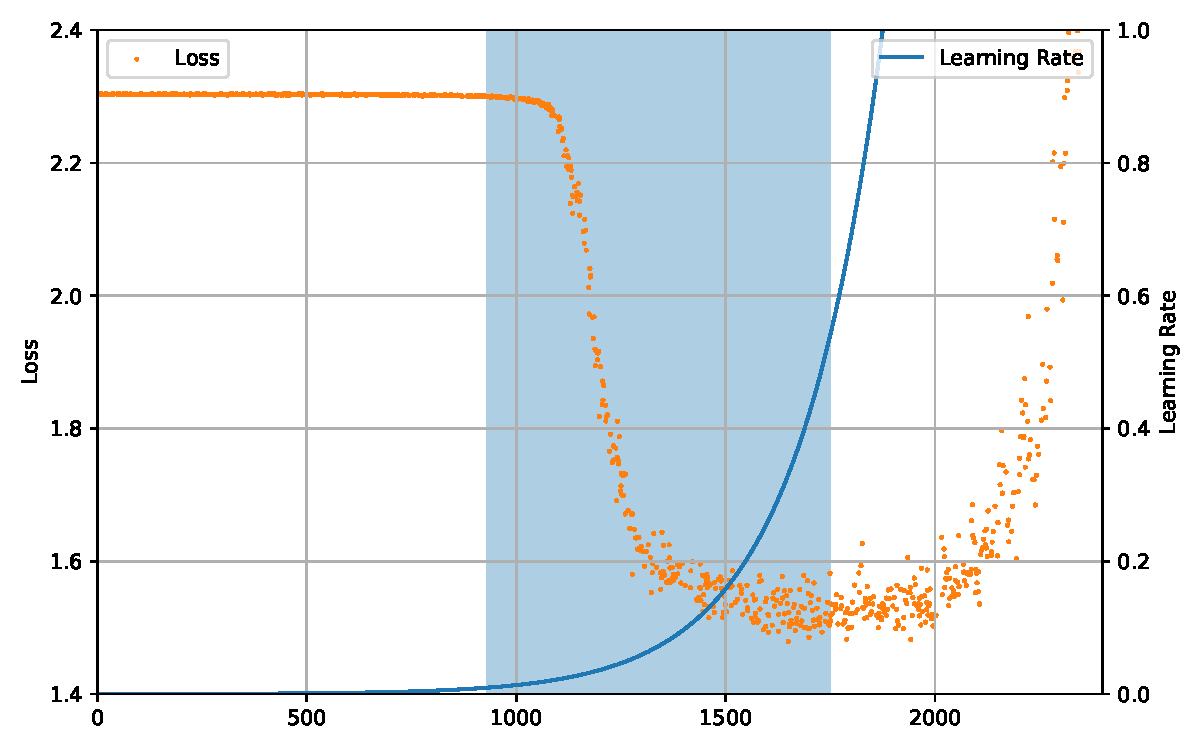
\includegraphics[scale=0.64]{images/lr_range_sgd.pdf}
    \caption{Learning rate with SGD optimizer}\label{fig:lr_range_sgd}
\end{figure}

\begin{figure}[ht!]
    \centering
    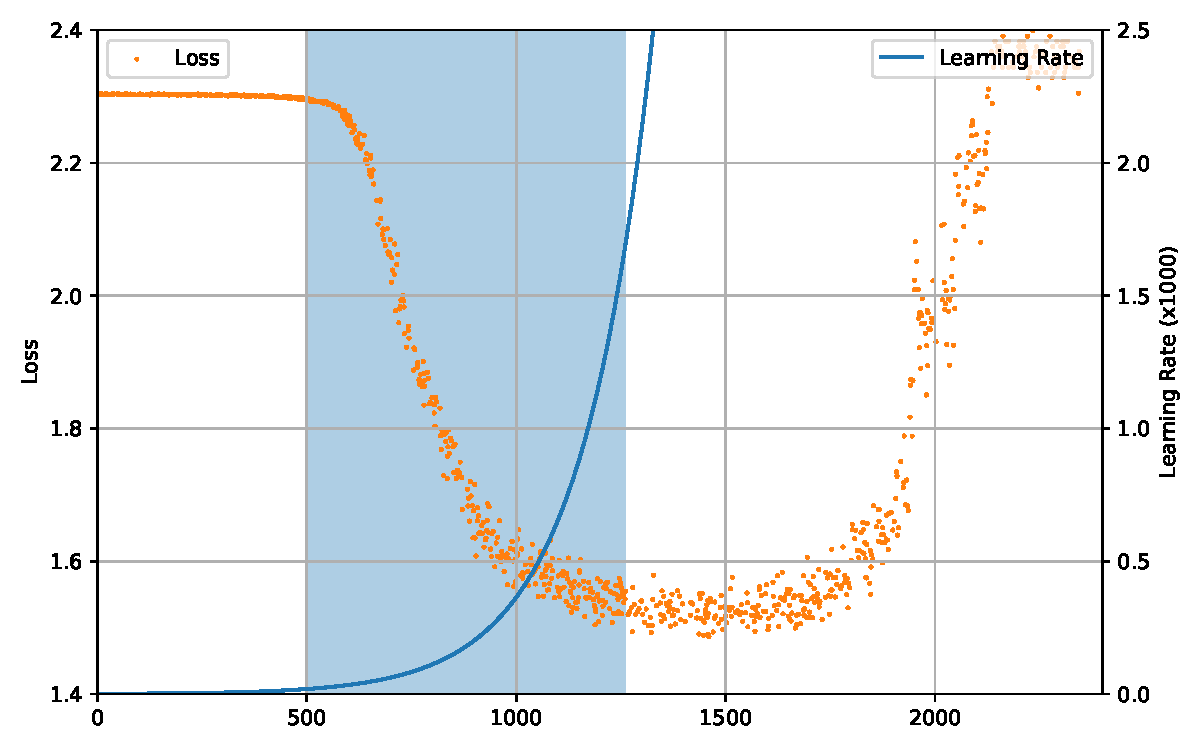
\includegraphics[scale=0.64]{images/lr_range_adam.pdf}
    \caption{Learning rate with Adam optimizer}\label{fig:lr_range_adam}
\end{figure}

\begin{figure}[ht!]
    \centering
    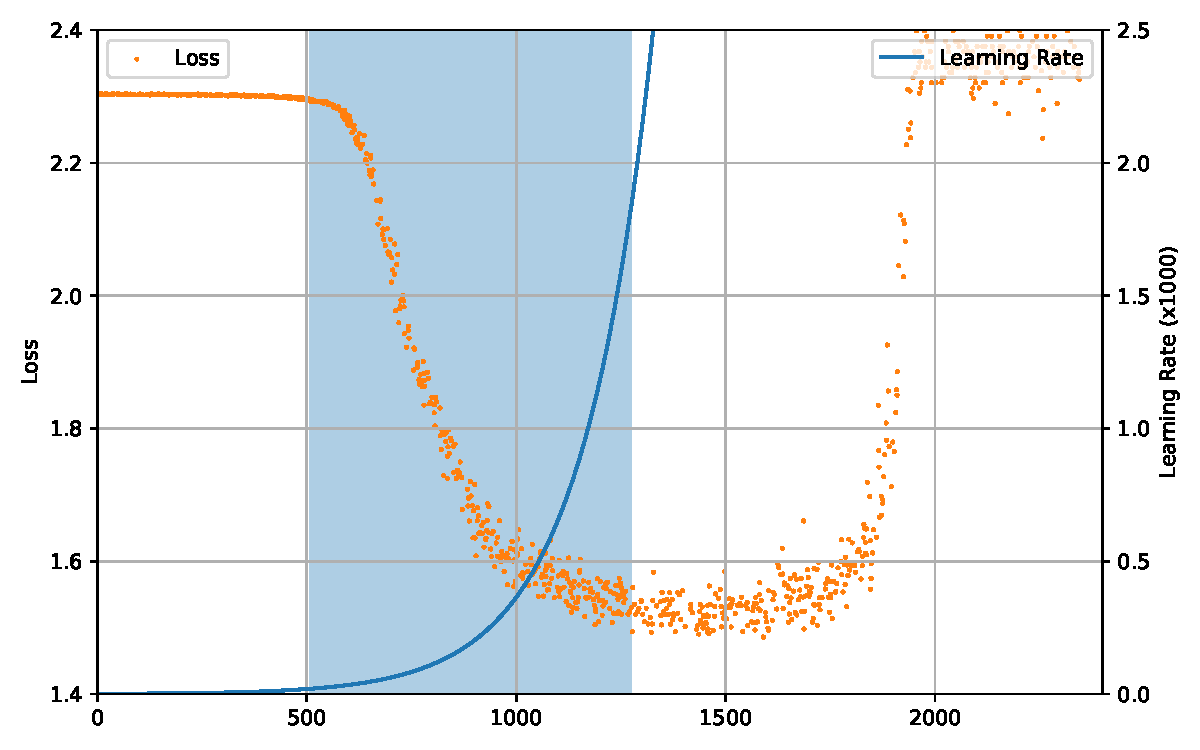
\includegraphics[scale=0.64]{images/lr_range_adamw.pdf}
    \caption{Learning rate with AdamW optimizer}\label{fig:lr_range_adamw}
\end{figure}

\begin{figure}[ht!]
    \centering
    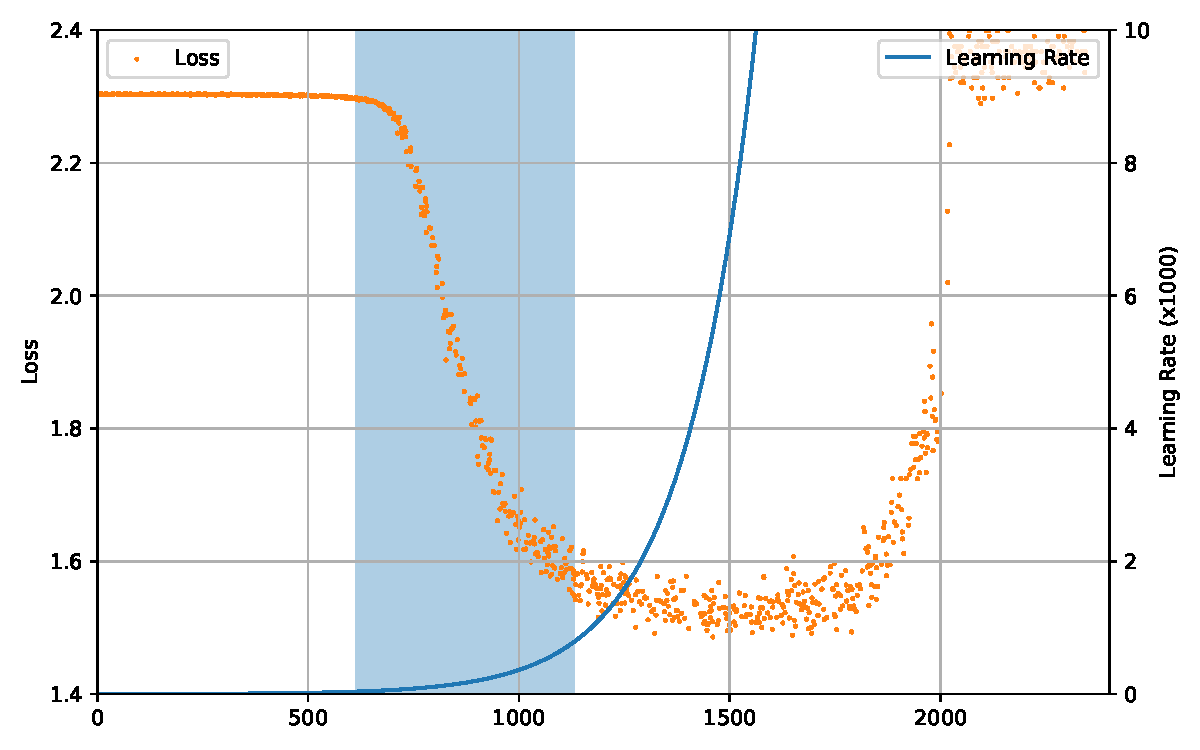
\includegraphics[scale=0.64]{images/lr_range_radam.pdf}
    \caption{Learning rate with RAdam optimizer}\label{fig:lr_range_radam}
\end{figure}

\clearpage
\section{LR Range Evaluation}



\end{document}
